%%%%%%%%%%%%%%%%%%%%%%%%%%%%%%%%%%%%%%%%%%%%%%%%%%%%%%%%%%%%%%%%%%%%%%
% All The Database Theory
%
% Compiled from the lectures of COMP 3005
% as taught by Lou Nel, at Carleton University
%
% Started: October 28, 2012
% By:      Simon Pratt
%%%%%%%%%%%%%%%%%%%%%%%%%%%%%%%%%%%%%%%%%%%%%%%%%%%%%%%%%%%%%%%%%%%%%%
\documentclass[11pt]{book}

\usepackage{geometry}
\geometry{verbose,tmargin=1in,bmargin=1in,lmargin=.5in,rmargin=.5in}
\usepackage[pdftex]{graphicx}
\usepackage{fancyhdr}
\usepackage{fix-cm}
\usepackage{amsmath}
\usepackage{enumerate}
\usepackage{amsthm}
\usepackage{amssymb}
\usepackage{parskip}
\usepackage{hyperref}
\usepackage{multicol}
\usepackage{nonfloat}

%%%%%%%%%%%%%%%%%%%%%%%%%%%%%%%%%%%%%%%%%%%%%%%%%%%%%%%%%%%%%%%%%%%%%%
% Extra stuff from John Howat
%%%%%%%%%%%%%%%%%%%%%%%%%%%%%%%%%%%%%%%%%%%%%%%%%%%%%%%%%%%%%%%%%%%%%%

\renewcommand{\implies}{\rightarrow}
\newcommand{\same}{\leftrightarrow}
\newcommand{\cross}{\times}
\newcommand{\xor}{\oplus}
\newcommand{\zz}{\mathbb{Z}}
\newcommand{\BigOh}[1]{O\!\left(#1\right)}
\newcommand{\LittleOh}[1]{o\!\left(#1\right)}
\newcommand{\BigOmega}[1]{\Omega\!\left(#1\right)}
\newcommand{\LittleOmega}[1]{\omega\!\left(#1\right)}
\newcommand{\BigTheta}[1]{\Theta\!\left(#1\right)}

%%%%%%%%%%%%%%%%%%%%%%%%%%%%%%%%%%%%%%%%%%%%%%%%%%%%%%%%%%%%%%%%%%%%%%
% Theorem, Lemma and Definitions
%%%%%%%%%%%%%%%%%%%%%%%%%%%%%%%%%%%%%%%%%%%%%%%%%%%%%%%%%%%%%%%%%%%%%%

\newtheorem{theorem}{Theorem}[chapter]
\newtheorem{lemma}{Lemma}[chapter]
\theoremstyle{definition}
\newtheorem{definition}{Definition}[chapter]
\newtheorem{claim}{Claim}[chapter]

%%%%%%%%%%%%%%%%%%%%%%%%%%%%%%%%%%%%%%%%%%%%%%%%%%%%%%%%%%%%%%%%%%%%%%
% Fix for amsthm and parskip
% URL: http://tex.stackexchange.com/questions/22119/how-can-i-change-the-spacing-before-theorems-with-amsthm
%%%%%%%%%%%%%%%%%%%%%%%%%%%%%%%%%%%%%%%%%%%%%%%%%%%%%%%%%%%%%%%%%%%%%%

\makeatletter
\def\thm@space@setup{%
  \thm@preskip=\parskip \thm@postskip=0pt
}
\makeatother

%%%%%%%%%%%%%%%%%%%%%%%%%%%%%%%%%%%%%%%%%%%%%%%%%%%%%%%%%%%%%%%%%%%%%%
% Header/footer
% Mostly taken from: 
%  https://texblog.wordpress.com/2007/11/07/headerfooter-in-latex-with-fancyhdr/
%%%%%%%%%%%%%%%%%%%%%%%%%%%%%%%%%%%%%%%%%%%%%%%%%%%%%%%%%%%%%%%%%%%%%%
\pagestyle{fancyplain}
\setlength{\headheight}{14pt}
\fancyhead{}             % clear header
\fancyfoot{}

\fancyhead[L]{All The Database Theory}
\fancyhead[C]{Page \thepage }
\fancyhead[R]{Simon Pratt}

%%%%%%%%%%%%%%%%%%%%%%%%%%%%%%%%%%%%%%%%%%%%%%%%%%%%%%%%%%%%%%%%%%%%%%
% Pretty math macros
%%%%%%%%%%%%%%%%%%%%%%%%%%%%%%%%%%%%%%%%%%%%%%%%%%%%%%%%%%%%%%%%%%%%%%
\newcommand{\summ}[2]{\ensuremath{\displaystyle\sum\limits_{#1}^{#2}}} 
%pretty summation

%%%%%%%%%%%%%%%%%%%%%%%%%%%%%%%%%%%%%%%%%%%%%%%%%%%%%%%%%%%%%%%%%%%%%%
% Relational Algebra
%%%%%%%%%%%%%%%%%%%%%%%%%%%%%%%%%%%%%%%%%%%%%%%%%%%%%%%%%%%%%%%%%%%%%%

\newcommand{\GoesTo}{$\leftarrow$ }
\newcommand{\Project}[1]{{\Huge\bf$\pi$}$_{\text{#1}}$}
\newcommand{\Select}[1]{{\Huge\bf$\sigma$}$_{\text{#1}}$}
\renewcommand{\Join}[1]{{\Huge\bf$\otimes$}$_{\text{#1}}$}
\newcommand{\CartesianProduct}{{\Huge\bf$\times$}}
\newcommand{\NaturalJoin}{{\Huge\bf$*$} }
\newcommand{\AggregateFunction}[1]{{\Huge\bf$f$}$_{\text{#1}}$}

%%%%%%%%%%%%%%%%%%%%%%%%%%%%%%%%%%%%%%%%%%%%%%%%%%%%%%%%%%%%%%%%%%%%%%
% Document
%%%%%%%%%%%%%%%%%%%%%%%%%%%%%%%%%%%%%%%%%%%%%%%%%%%%%%%%%%%%%%%%%%%%%%

\title{All The Database Theory}
\date{}
\author{Simon Pratt}

\begin{document}
\tableofcontents
\newpage
\begin{multicols}{2}
  
  \chapter{Functional Dependency}

\begin{definition}
Given a set of n-tuples $R$, we say that 
\end{definition}

  \chapter{Normal Forms}

\section{First Normal Form (1NF)}

\begin{definition}

A \emph{superkey} of a relation $S,R$ is a set of attributes $X$ such
that $t_1(X) = t_2(X)$ if and only if $t_1 = t_2$.  Such attributes
are said to be \emph{prime}.  

A superkey is said to be \emph{minimal} if it has the least number of
attributes required to meet this condition.  Such a minimal superkey
is called a candidate key.

\end{definition}

\begin{definition}

A set of relations is in \emph{First Normal Form} if every relation
has a minimal superkey.

\end{definition}

\section{Second Normal Form (2NF)}

\begin{definition}

A \emph{partial dependency} is a dependency of a non-prime attribute
on a proper subset of a candidate key.

\end{definition}

\begin{definition}

A set of relations is in \emph{Second Normal Form} if it is in 1NF and
it contains no partial dependencies.

\end{definition}

\section{Third Normal Form (3NF)}

\begin{definition}

A \emph{trivial dependency} is a dependency $X \rightarrow Y$ where $Y
\subseteq X$.

\end{definition}

\begin{definition}

A \emph{transitive dependency} is a dependency inferred from the
transitive axiom.  If $X \rightarrow Y$ is a transitive dependency, we
say $Y$ is \emph{transitively dependendent} on $X$, otherwise $Y$ is
\emph{directly dependent} on $X$.

\end{definition}

\begin{definition}

A set of relations is in \emph{Third Normal Form} if it is in 2NF and
all functional dependencies $X \rightarrow Y$ are trivial, or X is a
superkey, or all attributes $a \in (X - Y)$ are prime.

\end{definition}

\section{Boyce-Codd Normal Form (BCNF)}

\begin{definition}

A set of relations is in \emph{Boyce-Codd Normal Form} if it is in 2NF
and all functional dependencies $X \rightarrow Y$ are trivial or X is
a superkey.

\end{definition}

  \chapter{Relational Algebra}

Given a relation $(S,R)$, we define a formalism for retrieving
information.

\section{Select}

The \emph{selection} operator denoted \Select{} takes two paramters: a
set of attributes in $S$ and a relation $(S,R)$, and returns a new
relation $(S',R')$ in which $S'$ contains only the specified
attributes of $S$ and $R'$ contains modified tuples with only values
corresponding to the attributes of $S'$.  We denote this as
\Select{X}Y where X is the set of attributes to keep and Y is the
relation.

\section{Project}

The \emph{projection} operator denoted \Project{} takes two
parameters: a set of conditions on the attributes of $S$ and a
relation $(S,R)$, and returns a new relation $(S,R')$ where $R'
\subseteq R$ is the set of all tuples that meet the specified
conditions.  We donte this as \Project{X}Y where X is the set of
conditions and Y is the relation.

\section{Renaming Attributes}

It is often useful to rename attributes and save intermediate
relations.  We do this with the \GoesTo operator as in the following
example.

Stuff(Noms,NotNoms) \GoesTo \Select{Edibles,Inedibles} Items

This example selects the Edibles and Inedibles attributes of the Items
relation, and saves them to a new relation Stuff and rename the
attributes to Noms and NotNoms.

\section{Cartesian Product}

The \emph{Cartesian Product} binary operator denoted \CartesianProduct
takes relations $(S,R)$ and $(S',R')$ and returns the relation $(S
\cup S',R'')$ where $R''$ is a set of tuples $\{r r' | r \in R, r' \in
R' \}$.

\section{Natural Join}

The \emph{natural join} binary operator denoted \NaturalJoin takes
relations $(S,R)$ and $(S',R')$ where $J = S \cap S' \neq \emptyset$,
and returns $(S \cup S',R'')$ where $R''$ is the set of tuples $\{r r'
| r \in R, r' \in R', r(J) = r'(J) \}$.

\section{Join}

The \emph{join} operator denoted \Join{} takes relations $(S,R)$,
$(S',R')$, and a function $f$, and returns the relation $(S \cup
S,R'')$ where $R''$ is the set of tuples $\{ r r' | r \in R, r' \in
R', f(r,r') = true \}$.

For example:

CALL
\Join{CALL.portid = CALL\_FORWARD\_NUMBERS.portid}
CALL\_FORWARD\_NUMBERS

Joins CALL and CALL\_FORWARD\_NUMBERS when CALL.portid =
CALL\_FORWARD\_NUMBERS.portid.

\section{Aggregate Function}

The \emph{Aggregate Function} takes a set of attributes from the
relation, a function list, and a relation and returns the result of
applying the function to the tuples of the relation and grouping by
the given attributes.  Available functions are SUM, AVERAGE, MINIMUM,
MAXIMUM, COUNT.

For example:

lineid \AggregateFunction{count scode} SERVICE\_SUBSCRIBERS

Returns the count of unique values for attribute scode, grouped by
lineid on relation SERVICE\_SUBSCRIBERS.

  \chapter{Implementation}

Topics: disk blocks, hashing, and B+ trees.

Databases store data persistently on a hard disk, and since most hard
disks in use today are revolving magnetic disks, databases are highly
optimized for this.

Revolving magnetic disks, as opposed to solid state disks, have a
physical disk that spins under a moving read/write head.  Such disks
are organized into sectors (a slice of the disk), and each sector is
further divided into blocks of a fixed number of bytes.  In order to
read to or write a block in a sector of the spinning disk, both the
disk and head must move, which is the bottleneck in the speed of a
drive.

Databases are optimized for this scenario, in that they minimize the
number of blocks to be read from the drive, thus minimizing the amount
of disk and head movement.

\section{B+ Trees}

The biggest optimization to minimize block retrievals is to store as
much information within a block as possible.  A B+ tree is a tree with
a large branching factor wherein all data nodes are leafs.

In a B+ tree, a branching factor $b$ is specified and largely
determines the structure of the tree.  The branching factor $b$ is an
upper bound on the number of children each internal node can have.

The smallest possible B+ tree contains 2 nodes: the root node with one
child data node.  

If at any point the number of nodes pointed to by the root surpasses
the branching factor $b$, the nodes are split between two new internal
nodes to which the root now points.  Note that these nodes may be data
nodes as in the base case, or they may be internal nodes which may
themselves point to internal nodes or data nodes.




  \appendix
  \chapter{Entity Relational Diagrams}

Entity Relational Diagrams are a visual diagramming language for
describing entities using relational vocabulary.

To describe an entity, we draw a rectangle in which we write
emphasized on the first line the name of the entity, and on the
remaining lines the attributes of the entity.  

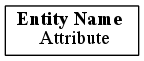
\includegraphics{figs/entity.png}

If it is a strong entity, we underline its natural key.  

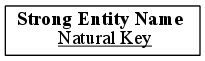
\includegraphics{figs/strong_entity.png}

If it is a weak entity, we dashed underline its discriminator (or weak
key), and draw a second rectangle around the first.

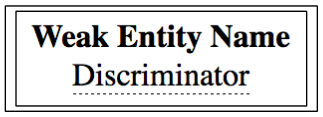
\includegraphics[scale=0.7]{figs/weak_entity.png}

A variation is to write the attributes in ovals connected to the
entity by lines.

To describe a relationship between two entities, we draw a rhombus in
which we write the name of the relationship.  We then draw lines
between the rhombus and the entities it relates.  We double the line
between an entity and the relationship if the entity can't exist
without being part of such a relationship.  We further decorate the
lines with cardinality: ``1'' meaning exactly one of this entity
relates to one or many of the other entity in the relationship, ``n''
meaning many of this entity relates to one or many of the other
entity, or we can specify minima and maxima by ``(min,max)''.  If the
relationship itself has attributes, they will be drawn in ovals
connected to the relationship by a line.

  \chapter{SQL}

SQL is a Data Definition Language (DDL) and a Data Manipulation
Language (DML), which means that SQL is suitable for both defining and
manipulating large amounts of data.


\end{multicols}
\end{document}
